\documentclass[UTF8]{mcmthesis}
    % \usepackage{ctex}           % 暂时需要中文时添加, 最后注释掉即可
    \mcmsetup {
        tcn = 2505974, problem = B,    %% tcn is team control number
        titleinsummary = true,             %% title appears on summary sheet
    }

    % 调整 \item 的间距 
    \usepackage{paralist}
    \usepackage{enumitem}
    \usepackage{hyperref}
    \hypersetup{
        colorlinks=true,
        linkcolor=black
    }
        \let\itemize\compactitem
        \let\enditemize\endcompactitem
        \let\enumerate\compactenum
        \let\endenumerate\endcompactenum
        \let\description\compactdesc
        \let\enddescriprion\endcompactdesc
    % 调整公式和正文的间距 (公式和正文更紧凑)
    \makeatletter
    \renewcommand\normalsize {
        % \@setfontsize\normalsize\@xpt\@xiipt
        \abovedisplayskip 5\p@ \@plus2\p@ \@minus5\p@
        \abovedisplayshortskip \z@ \@plus3\p@
        \belowdisplayshortskip 5\p@ \@plus3\p@ \@minus3\p@
        \belowdisplayskip \abovedisplayskip
        \let\@listi\@listI
    }
    \makeatother

    % \renewcommand{\baselinestretch}{1.2}      % 行间距
    \setlength{\parskip}{0.5em}                 % 段间距

    \usepackage{tikz}
        \usetikzlibrary{arrows} % 按需要添加扩展

    % 一般默认字体就好
    % \usepackage{mathptmx}     %% 数学公式罗马字体,对公式和正文都起作用
    % \usepackage{txfonts}      %% 数学公式罗马字体,对公式和正文都起作用
    % \usepackage{mathpazo}     %% COMAP 官方版物字体,对公式和正文都起作用
    % 一些重命名 ↓
    % \providecommand{\diff}{\mathop{}\!\mathrm{d}} %% 微分符号,正体 d
    % \providecommand{\me}{\mathrm{e}}              %% 无理数,正体 e
    % \providecommand{\mi}{\mathrm{i}}              %% 虚数单位,正体 i

    %% 设置目录节标题后加点
    \usepackage[titles]{tocloft}
    \renewcommand\cftsecdotsep{\cftdotsep}
    \renewcommand{\appendixpagename}{\Large\bfseries Appendices}

    %% 定制 Synopsis 页目录
    %% 根据需要把 Synopsis 改为 Memo or Handout 等等
    \fancypagestyle{Synopsis} {
        \fancyhf{}
        \lhead{\sffamily \team}
        \rhead{\sffamily Synopsis}
    }
    \title{\bfseries Title}  % 题目
  
\begin{document}
    \begin{summary}
        Lorem ipsum dolor sit amet consectetur adipisicing elit. Natus porro exercitationem magnam error non. Consectetur praesentium quaerat libero doloribus cumque ea? Veniam sapiente eum voluptatem omnis nostrum error iusto consequatur aspernatur perferendis ea sit architecto dolore, fugiat nam reiciendis accusantium! Voluptatum odio quis atque laboriosam. Vitae nemo aspernatur doloremque nam nulla, commodi earum architecto repellendus, odit doloribus hic deleniti facere praesentium aperiam accusamus? Perferendis dolorum dolor enim iste aperiam ipsam est voluptas modi neque minus architecto, consectetur delectus. Esse, incidunt.

        Lorem ipsum dolor sit amet consectetur adipisicing elit. A reiciendis quisquam nobis vel quos voluptatum, eum iusto vitae nam similique? Minus consequuntur placeat cupiditate itaque recusandae! Cupiditate quod, perspiciatis aliquid et ratione maxime temporibus aspernatur, accusamus nobis eaque illo culpa perferendis possimus sit eveniet iusto. Ea, culpa sapiente ullam delectus accusantium totam reprehenderit neque porro omnis dignissimos fugiat libero et harum beatae aperiam eligendi eaque dolor adipisci doloremque incidunt. Cum, deserunt ipsum. A dolorum ducimus suscipit. Culpa quos, quibusdam libero, pariatur quis asperiores commodi maxime dicta accusamus exercitationem qui ullam, illo natus velit praesentium quisquam nesciunt unde modi tenetur consequatur dolor doloremque esse. Repellat delectus quaerat illum obcaecati optio libero reprehenderit aliquid atque veritatis veniam quisquam, exercitationem perspiciatis sit laboriosam. Enim est exercitationem similique architecto eaque quis? Vero quod, nesciunt praesentium tempora excepturi voluptatibus saepe eveniet illum harum, officiis laborum optio perspiciatis. Dolore dolor laboriosam a quasi nulla vel deleniti.

        Lorem ipsum dolor sit amet consectetur adipisicing elit. Consectetur voluptatem, atque quaerat ratione maiores ab magnam eum neque nostrum pariatur, labore reprehenderit illum expedita perferendis optio nisi voluptates ducimus quam molestiae sed odit sunt! Corrupti tempore unde, delectus in excepturi exercitationem laborum ipsam nemo ad? Corrupti, totam, in, nemo dolorem doloribus neque harum exercitationem temporibus nulla est at saepe! Officia cumque, quo quibusdam rem, ipsam reprehenderit eos debitis inventore eaque minima, sunt tenetur labore ducimus nam voluptas accusamus exercitationem numquam ab ratione ad error. Fugiat qui nesciunt dignissimos tempore adipisci aliquam pariatur. Architecto asperiores pariatur voluptatum inventore dolorum dolor dolores?

        Lorem ipsum dolor, sit amet consectetur adipisicing elit. Quisquam quae minima, provident aperiam totam quaerat, commodi suscipit dicta maiores tempora accusantium error reprehenderit sunt placeat eaque dolores voluptates. Saepe nobis aliquam error dolore ex velit corporis fugit vel? Tenetur accusamus nam inventore fugiat, possimus deserunt eveniet pariatur incidunt maxime aspernatur?

        \textbf{Here is bold text}

        $$
        \begin{aligned}
        a & =b+c \\
        & =d+e
        \end{aligned}
        $$

    
        \vspace{2em}
        \noindent\textbf{Key Words: } KeyWord1; KeyWord2
    \end{summary}

    \maketitle
    \newpage
    \tableofcontents

    \newpage
    \setcounter{page}{1}
    \section{Introduction}
        \subsection{Problem Background}
            \hspace*{2em}Juneau, one of the most captivating tourist destinations in the United States, attracts visitors from around the world with its unique charm and natural beauty. Though only accessible by air and sea, the city’s allure remains irresistible to travelers.
            However, while tourism brings significant economic benefits, it also presents risks due to the fragile environmental resources and the potential for irreversible degradation. With a population of just under 30,000 residents, Juneau is already grappling with the strain of millions of tourists each year. To mitigate these impacts, immediate measures are needed to ensure sustainable tourism and enhance both the safety and well-being of the local community.
            
            Therefore, it is crucial to assess the true impact of tourism on the city. By adopting a science-based and rational approach, we can foster economic growth while preserving Juneau’s biodiversity and ecological integrity. Policymakers and the tourist council will benefit from reliable methods to measure how best to manage visitor numbers and allocate public funds to support community programs.
            
            In this paper, we will focus on key factors that influence sustainable tourism, examining their impact on key indicators. Additionally, based on our findings, we will provide long-term, generalized management recommendations that can be applied to other destinations facing overtourism challenges.

            \begin{figure}[htbp]
                \centering
                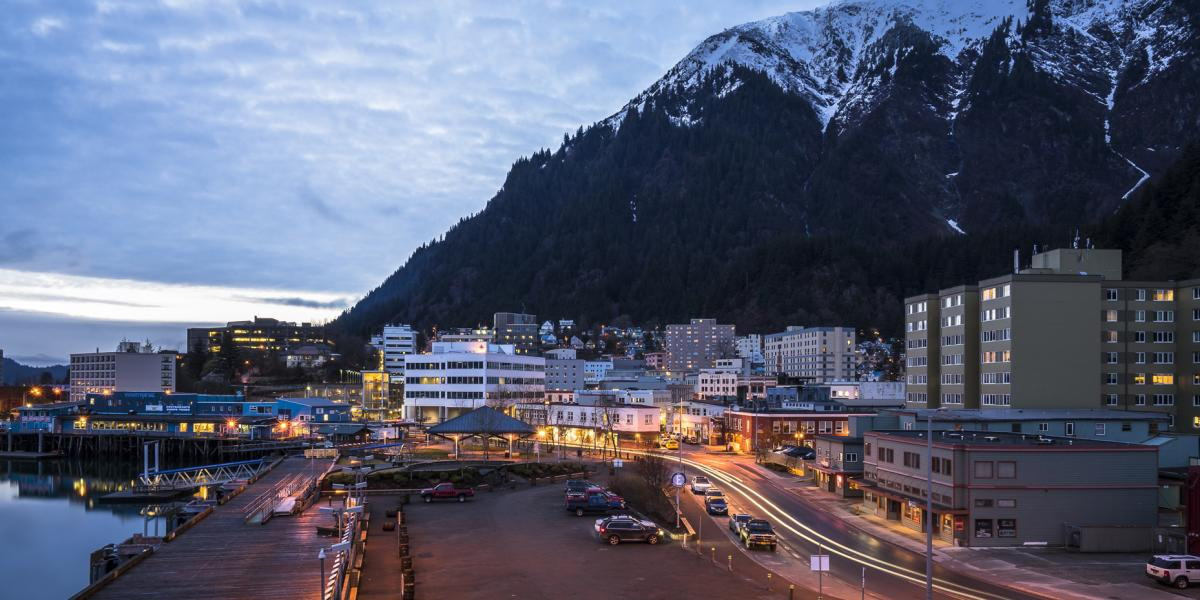
\includegraphics[width=8cm]{figure1.png}
                \caption{Dawn View of Juneau}
            \end{figure}
        
        \subsection{Restatement of the Problem}
        \hspace*{2em}Juneau is a famous toursism cities with many complexities and risks. Through in-depth analysis and research on the factors of the problem, combined with the specific constraints given, the restate of the objectives can be expressed as follows:


   
           \textbf{Objective 1:} Analyze the specificities of different areas and formulate specific policies and management strategies tailored to the needs of each area.
            
           \textbf{Objective 2:} Develop a comprehensive analytical method to evaluate and rank different policies and strategies, considering the animal-human interactions and economic impacts.
           
           \textbf{Objective 3:} Project and assess the long-term ecological and economic situation in the Maasai Mara by utilizing the proposed optimal management strategies.
           
           \textbf{Objective 4:} Considering the results obtained above, provide a two-page non-technical report for the Kenya Tourism and Wildlife Commission.

        \subsection{Overview of Our Works}
        \hspace*{2em} Based on the comprehensive review of the existing reports and data, our work mainly includes the following:

            \begin{enumerate}
                \item  We begin by building a model to evaluate the environmental status and quantify its factors. The environmental status is estimated by the area of one of the most significant ecosystem - glaciers. 
                \item We develop an assesment model. Take the economic gain as divese factors. Next we introduce a method to re-revaluate the satisfaction of residents as another factor to consider. By computing, we successfully approached (econimicn gain),E(environment status),S(satisfaction index).
                \item We conduct a multiple-objective-programming analysis, for opitimizing all considerd factors, including neccessary constraints, thus getting a reseanble values that can be optimized for enacting managements.
                \item We choose Beijing and Vatican as another tourist destinations impacted by  overtourism to adapt our model. We analysised their features, found out the similarities and differences. Based on a sectoral perspective, we used the same model to evaluate the sustainbale toursim condition for the two cities.
                
            \end{enumerate}
            

    \section{Assumptions}

                \hspace*{2em}\textbf{Assumption 1: Animals naturally increase at the same rate every year.} \\
                \hspace*{2em} \(\Rightarrow\) \textbf{Justification:} Though the ecnomic growth of the world happens each year, so is the inflation rate growing at a similar rate. What's more, people tend to make budget and have constant consumption habits.\\
                
                \textbf{Assumption2: The tourist council can totally control the number of toursists each year but no more than the highest level.} \\
                \hspace*{2em} \(\Rightarrow\) \textbf{Justification:} In this model, we assume that there is always overtourism problem, so the officers of the council can limit the numbers of tourists by issuing polices. It is also a fact that in 2020, no more than 100 people travelled at Juneau.\\
                
               \textbf{Assumtion3: the ratio  of tourists on a cruise ship to the total number of tourists is nearly constant.} \\
                \hspace*{2em} \(\Rightarrow\) \textbf{Justification:} In this model, we disregard the fact that this ratio changes since it is relatively uncorrelated to our proect.\\
                
                \textbf{Assumption 4: The data collected can be considered reliable and reflect the state of the natural environment.} 
        \\        \hspace*{2em} \(\Rightarrow\) \textbf{Justification:} we searech for data from reliable resoucres with high accuracy.
    \section{Notation}
        \hspace*{2em}Important notations used in this paper are listed in the table \ref{tab:notations}.
        \vspace{-.5em}
        \begin{table}[htbp]
            \centering
            \caption{Notations}
            \vspace{0.5em}
            \begin{tabular}{cc}
                \toprule                % 顶部线
                    \textbf{Symbols} & \textbf{Description} \\ 
                \midrule                % 中部线
                $I$        & Total tourism revenue of Juneau every year \\ 
                $V$        & The total number of tourists every year \\ 
                $s$        & Per capita spending by tourists \\ 
                $r$        & tax rate related to tourism \\  
                $B$        & Additional revenue of tourism \\ 
                $E$        & Environmental status, as indicated by glacier area \\ 
                $\mu$      & Environmental damage per dollar spent by tourists \\ 
                $\delta$   & Self-healing coefficient of the environment  \\ 
                $g$        & Environmental governance effect per dollar used by government \\ 
                $k$        & Proportion of additional revenue invested in glacier protection \\ 
                $G$        & Economic gain \\ 
                $a$        & Jobs created per tourist \\ 
                $S$        & Resident Satisfaction \\  
                \bottomrule             % 底部线
            \end{tabular}
            \label{tab:notations}
        \end{table}
        \begin{table}[h!]
            \centering
            \begin{tabular}{|c|l|}
            \hline
            \textbf{Symbol} & \textbf{Description} \\ \hline
            $I$        & Total tourism revenue of Juneau every year \\ \hline
            $V$           & The total number of tourists every year \\ \hline
            $s$           & Per capita spending by tourists \\ \hline
            $B$           & Additional revenue of tourism \\ \hline
            $E$             & Environmental status, as indicated by glacier area \\ \hline
            $\mu$             & Environmental damage per dollar spent by tourists \\ \hline
            $\delta$             & Self-healing coefficient of the environment  \\ \hline
            $g$           & Environmental governance effect per dollar used by government \\ \hline
            $k$             & Proportion of additional revenue invested in glacier protection \\ \hline
            $G$        & ecnomic gain \\ \hline
            $A$             & Economic income of local residents \\ \hline
            \end{tabular}
            \caption{Symbol Descriptions}
            \label{tab:symbol_descriptions}
            \end{table}
            

    \section{Problem 1}
    \begin{figure}[htbp]
        \centering
        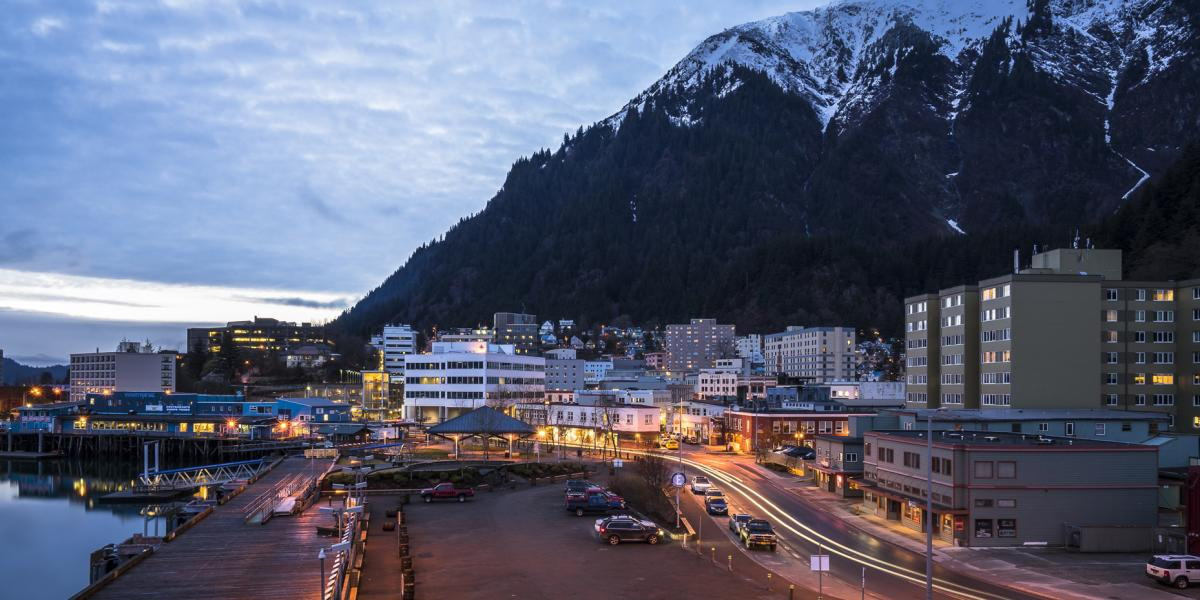
\includegraphics[width=8cm]{figure1.png}
        \caption{114514}
    \end{figure}
    \section{Problem 2}
    \section{Problem 3}
    \section{Results}
    \section{Model Evaluation}
        \subsection{Strengths}
diangun
            
        \subsection{Weaknesses}
            \begin{enumerate}
                \item 
            \end{enumerate}


    %\label{LastPage2}
    \addcontentsline{toc}{section}{References}
        \begin{thebibliography}{99}
            \bibitem{link}
            Steven J. Leon.
            Linear Algebra with Applications.
            China Machine Press, 51 (2019).
        \end{thebibliography}


    \begin{appendices}
        Here are simulation programmes we used in our model as follow.
        
        \vspace{.5em}
        \noindent(1)\quad \verb|hello.cpp|
        \vspace{.5em}
        \begin{lstlisting}[language = c++, numbers = left]
    #include <iostream>
    int main() {
        std::cout << "Hello, world!\n";
        return 0;
    }
        \end{lstlisting}

    \end{appendices}
\end{document}
